\documentclass[12pt,UTF8,AutoFakeBold]{article}
\usepackage[a4paper]{geometry}
\usepackage[myheadings]{fullpage}
\usepackage{fancyhdr}
\usepackage{lastpage}
\usepackage{graphicx, wrapfig, subcaption, setspace, booktabs}
\usepackage{float}
\usepackage[T1]{fontenc}
\usepackage[font=small, labelfont=bf]{caption}
\usepackage{fourier}
\usepackage[protrusion=true, expansion=true]{microtype}
\usepackage[english]{babel}
\usepackage{sectsty}
\usepackage{url, lipsum}
\usepackage{tgbonum}
\usepackage{hyperref}
\usepackage{xcolor}
\usepackage{amsmath}
\usepackage[UTF8, scheme=plain, punct=plain, zihao=false]{ctex}
\usepackage{fontspec}
\usepackage{libertine}
\usepackage{pgf} % for the calculation
% \libcirc and \libcircblk display their '0' if the parameter is out of range
\newcommand{\libcirc}[1]{\pgfmathparse{
    ifthenelse(#1 > 0 && #1 < 21, Hex(9311+#1), Hex(9450)
    }\libertineGlyph{uni\pgfmathresult}}
\newcommand{\libcircdbl}[1]{\pgfmathparse{Hex(9460+#1)}\libertineGlyph{uni\pgfmathresult}}
\newcommand{\libcircblk}[1]{\pgfmathparse{
    ifthenelse(#1 > 0 && #1 < 11, Hex(10101+#1),
        ifthenelse(#1 > 10 && #1 < 21, Hex(9450-10+#1),
            Hex(9471)
        )
    )
    }\libertineGlyph{uni\pgfmathresult}}

\newcommand{\juncirc}[1]{{\fontspec[Ligatures=Discretionary]{Junicode}[#1]}}
\newcommand{\juncircdbl}[1]{{\fontspec[Ligatures=Discretionary]{Junicode}[[#1]]}}
\newcommand{\juncircblk}[1]{{\fontspec[Ligatures=Discretionary]{Junicode}<#1>}}

\makeatletter
\@addtoreset{equation}{section}
\makeatother

\newcommand{\HRule}[1]{\rule{\linewidth}{#1}}
\onehalfspacing
\setcounter{tocdepth}{5}
\setcounter{secnumdepth}{5}
\setmainfont{Times New Roman}%fontspec下这个命令设置全局默认字体


%-------------------------------------------------------------------------------
% HEADER & FOOTER
%-------------------------------------------------------------------------------
%-------------------------------------------------------------------------------
% TITLE PAGE
%-------------------------------------------------------------------------------

\begin{document}
\fontfamily{cmr}\selectfont
\title{ \normalsize \textsc{}
		\\ [2.0cm]
		\HRule{0.5pt} \\
		\LARGE \textbf{\uppercase{Deep Learning}
		\HRule{2pt} \\ [0.5cm]
		\normalsize \today \vspace*{5\baselineskip}}
		}

\date{}

\author{
		Zhihua Zhang (张志华)\\ 
		Ruohua Shi (史若画)\\
		Deap Learning Courses in Peking University}

\maketitle
\newpage
\tableofcontents
\newpage
%-------------------------------------------------------------------------------
% Section title formatting
\sectionfont{\scshape}
%-------------------------------------------------------------------------------

%-------------------------------------------------------------------------------
% BODY
%-------------------------------------------------------------------------------


\section{Overview}
\subsection{\textbf{Refrences}}

《Numerical Linear Algebra》\\
《Linear Algebra and Learning from Data》 \(https://math.mit.edu/~gs/learningfromdata/\) \\
《Numerical Optimization》\(http://www.bioinfo.org.cn/~wangchao/maa/Numerical_Optimization.pdf\) \\
\(https://github.com/ShiqinHuo/Numerical-Optimization-Books\)

\subsection{Machine Learning}

{\kaishu1)频率派/贝叶斯派}

    贝叶斯派的MCMC是目前最常用的采样方法,但是其计算问题仍需解决\\
{\kaishu2)参数化/非参数}

    参数化是指参数的数量和数值不依赖于数据,是固定的,如一个高斯分布就两个参数。
    
    非参数指参数的数量和数值依赖于数据,如最近邻算法,数据的个数就是参数的个数。
    
    kernel方法:这种方法可以将参数与非参数方法转化,“主问题->对偶问题”就是一种“参数->非参数”的方法。\\
{\kaishu3)生成模型/判别模型}

    \((x,y)\sim{\mathbb{D}}\),\(x\)和\(y\)服从联合分布。----生成模型
    
    \((x,y), y\sim{\mathbb{D}}\),\(x\)固定,指关注\(y\)的分布。----判别模型
    
\newpage

\newpage
\section{Chapter 2  Basics}
\subsection{Optimization Target}
对于一个分类器classification \(h\), 它的泛化误差{\textbf{The general error}} 定义为:
\begin{gather}
Pr(h(x)=y(x)) = \mathbb{E}_{x\in{\mathbb{D}}}(1_{(h(x)\not{=}y(x))})
\end{gather}
对分类问题 Classification:Input: \(x\in{R^{d}}\).  Output: \(y\in{\{-1,1\}}\)\\
对回归问题 Regression: Input: \(x\in{R^{d}}\).  Output: \(y\in{{R}}\)\\
已知一个训练数据序列: \({(x_i,y_i), i=1...n}, x_i\in{R^d}, y_i\in{\{-1,1\}}\),它的经验误差 {\textbf{the experience error of \(h\)}} 定义为:
\begin{gather}
\widehat{R}(h) = \mathbb{E}_{x\in{\mathbb{D}}}(1_{(h(x)\not{=}y(x))})\\
\widehat{D} = \frac{1}{n}\sum _{i=1}^{n}{{\delta}_{{x}_{i}}()}
\end{gather}
为了最小化这个经验误差,自然的得到一个{0-1 loss},它是高维不连续的,在数据量较大的时候很难做离散的梯度下降来优化。所以需要找到一个损失函数来代替,这个损失函数需要满足两点:1)凸函数(Convex);2)是一个上界函数(Upper bound of the original loss)。

\subsection{Basic Models}

{\bfseries\kaishu SVM logistic regression}

目标是\(max\{0,1-y_{i}w^{T}x_{i}\}\),多层的感知机就是一个嵌套的过程\(f()=f_{1}(f_{2}(...))\).\\
{\bfseries\kaishu Linear Classification}

首先做一个仿射函数(Affine Function):
\begin{gather}
L_{d} = \{f_{w,b}, w\in{R^d}, b\in{R}\}\\
f_{w,b}(x) = <w,x> + b = \frac{1}{n}\sum _{i=1}^{n}{w_{i}x_{i} + b_i}= <\bar{w},\bar{x}> \doteq <w,x>
\end{gather}

其中\(\bar{w} = (b,w)\in{R^{d+1}}\); \(\bar{x} = (1, x^{T})\in{R^{d+1}}\). \(h\)是 在\(L_d\)上的映射\(R\rightarrow y\). 对回归问题:\(h(x)=f_w(x)\),对分类问题:\(h(x)=sign(f_w(x))\)。\\

\textbf{【生成模型】 Generation Model}

对p维数据\((x,y)\),\(P(x,y)=(P(y)(P(x|y)\),设y的先验是伯努利分布,\(y\in{\{0.1\}}\),x服从正态分布。
\begin{gather}
P(y|\pi)=\pi^{y}(1-\pi)^{-y}; \pi\in(0,1)\\
P(x|y=0)=\frac {1}{{(2\pi)}^{p/2}{\left|\Sigma\right|}^{1/2}}exp\{ -\frac{1}{2}{(x-{\mu}_{0})}^{T}{\Sigma}^{-1}{(x-{\mu}_{0})}\}\\
P(x|y=1)=\frac {1}{{(2\pi)}^{p/2}{\left|\Sigma\right|}^{1/2}}exp\{ -\frac{1}{2}{(x-{\mu}_{1})}^{T}{\Sigma}^{-1}{(x-{\mu}_{1})}\}
\end{gather}
接下来做极大似然估计\(min-\sum_{i=1}^{n}{logP({y}_{i})} P(x_{i}|{y}_{i})\).假设已知求得的所有参数极大似然估计\({\hat{\theta}}_{MLE}\).那么去求y属于那一类其实就是求对\(y=0/1\)的后验概率,如果大于1/2则属于这一类。
\begin{equation}
\begin{aligned}
P(y=1|x,\theta)&=\frac{P(x|y=1)P(y=1|\pi}{P(x|y=1,\theta )P(y=1|\pi)+P(x|y=0,\theta )\cdot P(y=0|\pi)} \\
&=\frac{\pi exp {\{ -\frac{1}{2} {(x-\mu_1)}^{T}\Sigma}^{-1}{(x-\mu_1))\}}} {\pi exp \{-\frac{1}{2}{(x-\mu_1)}^{T}\Sigma^{-1}(x-\mu_1)\}+(1-\pi)exp\{-\frac{1}{2} {(x-\mu_0)}^{T} \Sigma^{-1}(x-\mu_0)\}}\\
&=\frac{1}{1+\frac{1-\pi}{\pi}exp \{ {(x-\mu_1)}^{T} {\Sigma}^{-1} (x-\mu_1)-{(x-\mu_0)}^{T} {\Sigma}^{-1}(x-{\mu}_{0})\}}\\
&=\frac{1}{1+exp\{-{({\mu}_{1}-{\mu}_{0}}^{T}{\Sigma}^{-1}x+\frac{1}{2}{({\mu}_{1}-{\mu}_{0})}^{T}{\Sigma}^{-1}({\mu}_{1}+{\mu}_{0})-log\frac{\pi}{1-\pi}\}}\\
&=\frac{1}{1+exp\{-w^Tx+b\}} \\
&w = \Sigma^{-1}(\mu_1-\mu_0); b=log\frac{\pi}{1-\pi}
\end{aligned}
\end{equation}
由上可知,\(P(y=1|x,\theta)>\frac{1}{2}\)与\(sign(w^Tx+b)\)一致。但是参数量减少了很多。\\
\textbf{【感知算法】 Perception Algorithm}
\\
1. Batch Perception 批处理(Mini Batch)\\

Input: \(\{(x_i,y_i)\}\)

Initialize: \(w^{(0)}=(0,...,0)\)

\(for \quad t=0,1,...,T\)

\(\quad if (\exists i, s.t. y_i<w^{(t)}, x_i>\le 0) \quad w^{(t+1)}=w^{(t)}+y_ix_i\)

\(\quad else \quad output w^{(t)} \)


\begin{equation}
\begin{aligned}
y_t<w^{(t+1)},x_t>&=y_i<w^{(t)}+y_tx_t,x_t>\\
&=y_i<w^{(t)},x_t>+{y_t}^2<x_t,x_t>\\
&=y_t<w^{(t)},x_t>+{\left\| x_t \right\|}^2
\end{aligned}
\end{equation}\\
\\
\textbf{2. Online Perception Algorithm}\\

Initialize: \(w^{(0)}=(0,...,0)\)

\(for \quad t=0,1,...,T\)

\(\quad Receive \quad x_t\)

\quad Predict \(C_r = sign(<w^{(t)},x_t>)\)

\(\quad if (y_t<w^{(t)}, x_i>\le 0) \quad w^{(t+1)}=w^{(t)}+\eta y_tx_t\)  \(\eta \in [0,1]\)

\(\quad else \quad w^{(t+1)}=w^{(t)} \)

现在我们的损失函数\(1_{[y<w,x>\le 0]}\)(Fig.\ref{fig1})替换成\(max\{0, -y<w,x>\}\)(\(max\{, -z\}\))(Fig.\ref{fig2})。这时由一个不连续的函数变成连续但不可导的函数。这时的优化目标变成\(min\{y(w)=\frac{1}{n}\sum _{n}^{i=1}{max\{0, -y_i<w_i,x_i>\}} \}\). 虽然零点处不可导,但是可以用此梯度来代替,参数更新过程是:

\(w^{ (t+1) }=w^{ (t) }+\eta { \nabla  }_{ w }y({ w }^{ (t) })\)

\(w^{ (t+1) }=w^{ (t) }-\eta { \nabla  }_{ w }y({ w }^{ (t) }),\quad if\quad <w^{ (t) },{ x }_{ t }>\neq 0\)

\(w^{ (t+1) }=w^{ (t) }+\eta { y }_{ t }{ x },\quad if\quad <w^{ (t) },{ x }_{ t }>=0\)
\({{\nabla}_{w}y({w})=-y}_{t}{x}_{t},\quad if\quad {y}_{t}(w^{(t)})<0\)

\({\nabla}_{w}y({w})=0, \quad \quad if\quad {y}_{t}(w^{(t)})>0\)

如果将拐点右移,如Fig.\ref{fig3}蓝色曲线,优化过程转为\(max\{0, 1-y<w,x>\}\),是SVM的优化过程,也就是到Hinton Loss。
\begin{figure}[htbp]
\centering
\begin{minipage}[t]{0.3\textwidth}
\centering
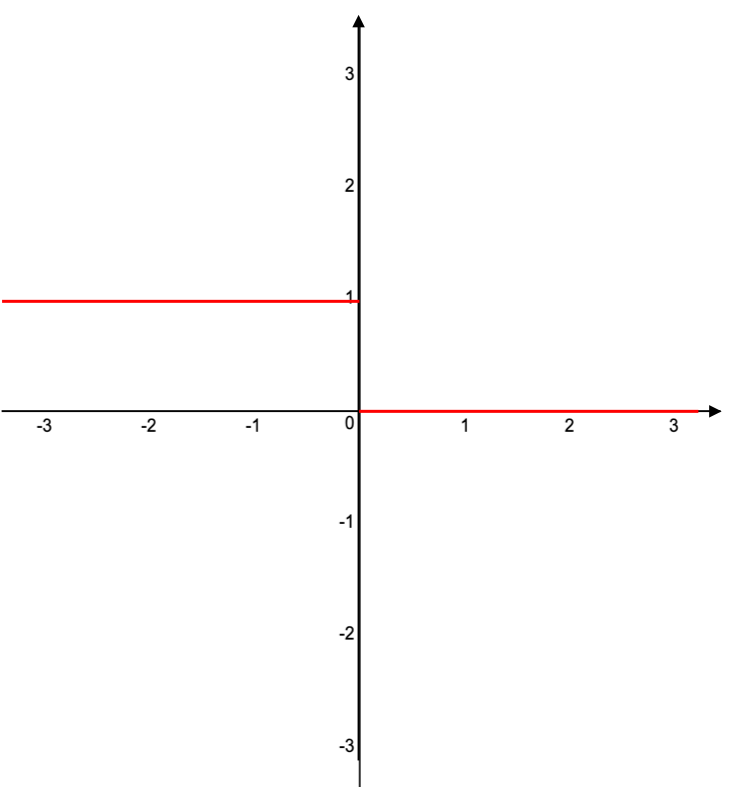
\includegraphics[width=4.5cm]{figs/0-1.png}
\caption{0-1 Loss}
\label{fig1} 
\end{minipage}
\begin{minipage}[t]{0.3\textwidth}
\centering
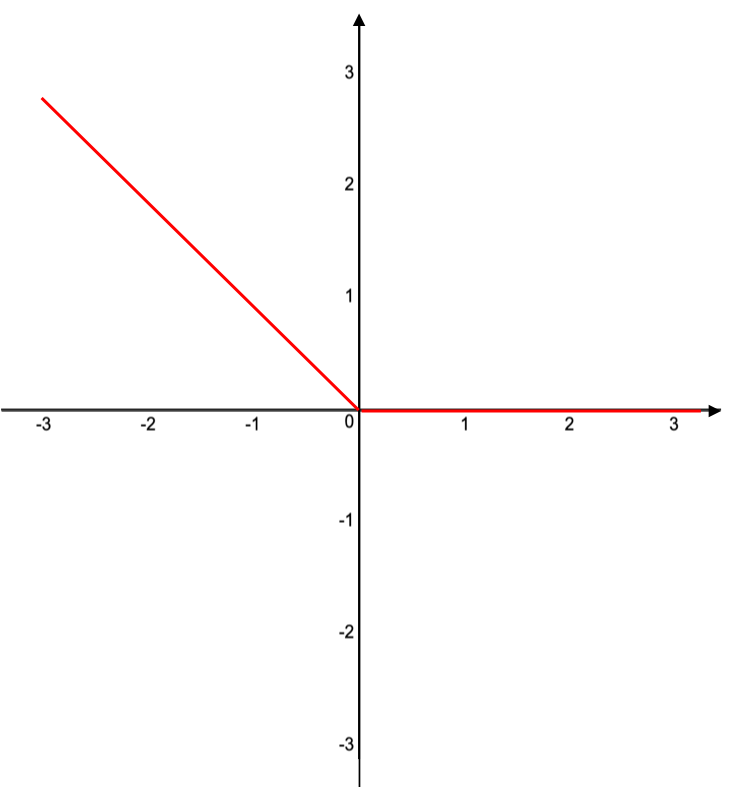
\includegraphics[width=4.5cm]{figs/-z.png}
\caption{Replace Loss}
\label{fig2} 
\end{minipage}
\begin{minipage}[t]{0.3\textwidth}
\centering
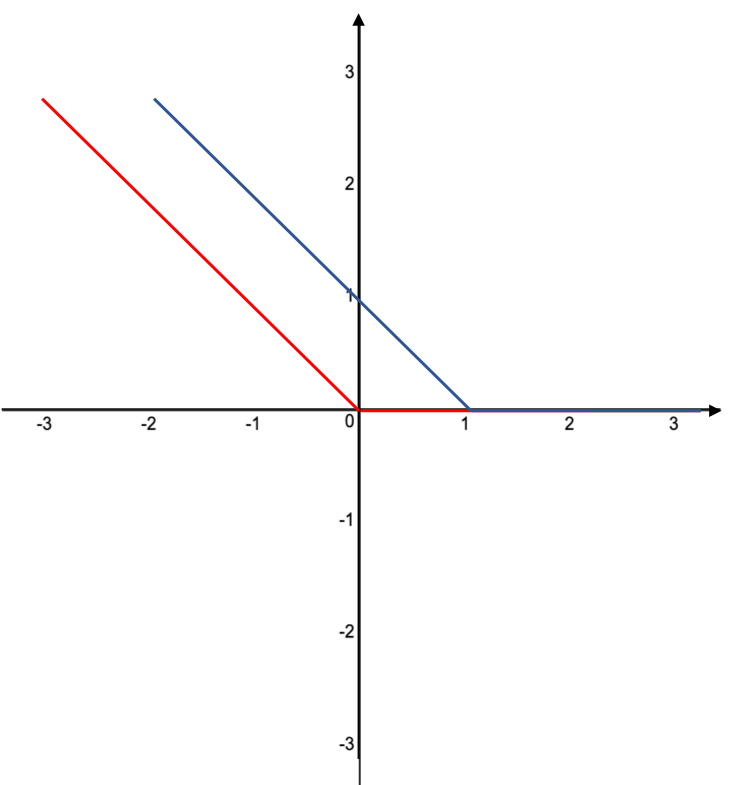
\includegraphics[width=4.5cm]{figs/hinton.png}
\caption{Hinton Loss}
\label{fig3} 
\end{minipage}
\end{figure}

\subsection{About Derivation}
\textbf{1. 梯度下降法}


定义导数和次导数:

\begin{gather}
\begin{aligned}
& { w }^{ (t+1) }={ w }^{ (t) }-\eta \nabla g({ w }^{ (t) })\\ 
& { w }^{ (t+1) }=\left\{
\begin{aligned}
             \begin{aligned}  
             &{ w }^{ (t) }-\eta \nabla g({ w }^{ (t) }),\quad \quad if\quad <{ w }^{ (t) },{ x }_{ t }>\neq 0.  \\  
             &{ w }^{ (t) }+\eta { { y }_{ t }x }_{ t },\quad \quad \quad \quad if\quad <{ w }^{ (t) },{ x }_{ t }>=0.\\ 
             \end{aligned}  
\end{aligned}
\right.\\
& \eta \nabla g({ w })=\left\{
\begin{aligned}
             \begin{aligned}  
             &-yx_t,\quad \quad if\quad y_t<w ,{ x }_{ t }< 0.  \\  
             &0,\quad \quad \quad \quad if\quad y_t<w ,{ x }_{ t }> 0.\\ 
             \end{aligned}  
\end{aligned}
\right.
\end{aligned}
\end{gather}

\textbf{2. 判别模型}

对$y\in \{0,1\}$,有:

\begin{gather}
\begin{aligned}
& P(x,y)=P(y)P(x|y)\\ 
& P(y|\pi )={ \pi  }^{ y }{ (1-\pi ) }^{ 1-y }\quad \quad \pi \in (0,1)\\ 
& P(x|y=0)=\frac { 1 }{ { (2\pi ) }^{ p/2 }{ \left| \Sigma  \right|  }^{ 1/2 } } exp\{ -\frac { 1 }{ 2 } { (x-{ \mu  }_{ 0 }) }^{ T }{ \Sigma  }^{ -1 }{ (x-{ \mu  }_{ 0 }) }\} \\ 
& P(x|y=1)=\frac { 1 }{ { (2\pi ) }^{ p/2 }{ \left| \Sigma  \right|  }^{ 1/2 } } exp\{ -\frac { 1 }{ 2 } { (x-{ \mu  }_{ 1 }) }^{ T }{ \Sigma  }^{ -1 }{ (x-{ \mu  }_{ 1 }) }\}
\end{aligned}
\end{gather}

模型的参数为$\pi, {\mu}_0, {\mu}_1, \Sigma $,已知数据对为$\{(x_i,y_i)\},i=1,...,N$,
\begin{gather}
\begin{aligned}
& \prod _{ n=1 }^{ N }{ P({ x }_{ i },{ y }_{ i })=\prod _{ n=1 }^{ N }{ P({ y }_{ i }) }  } P({ x }_{ i }|{ y }_{ i })\\
&P(y=1|x,\theta)=\frac{P(x|y=1)P(y=1|\pi}{P(x|y=1,\theta )P(y=1|\pi)+P(x|y=0,\theta )\cdot P(y=0|\pi)} \\
& min-\sum _{ n=1 }^{ N }{ log } P({ y }_{ i })P({ x }_{ i }|{ y }_{ i })\quad \quad \quad { \hat { \theta  }  }_{ MLE }
\end{aligned}
\end{gather}

\begin{equation}
\begin{aligned}
&=\frac{\pi exp {\{ -\frac{1}{2} {(x-\mu_1)}^{T}\Sigma}^{-1}{(x-\mu_1))\}}} {\pi exp \{-\frac{1}{2}{(x-\mu_1)}^{T}\Sigma^{-1}(x-\mu_1)\}+(1-\pi)exp\{-\frac{1}{2} {(x-\mu_0)}^{T} \Sigma^{-1}(x-\mu_0)\}}\\
&=\frac{1}{1+\frac{1-\pi}{\pi}exp \{ {(x-\mu_1)}^{T} {\Sigma}^{-1} (x-\mu_1)-{(x-\mu_0)}^{T} {\Sigma}^{-1}(x-{\mu}_{0})\}}\\
&=\frac{1}{1+exp\{-{({\mu}_{1}-{\mu}_{0}}^{T}{\Sigma}^{-1}x+\frac{1}{2}{({\mu}_{1}-{\mu}_{0})}^{T}{\Sigma}^{-1}({\mu}_{1}+{\mu}_{0})-log\frac{\pi}{1-\pi}\}}\\
&=\frac{1}{1+exp\{-w^Tx+b\}} \Leftrightarrow sign(w^Tx+b)
\end{aligned}
\end{equation}

\textbf{2. 生成模型}

已知数据$(x,y),x\in R^p, y\in\{0,1\},\{-1,1\}$
\begin{gather}
\begin{aligned}
& P(x,y)=P(y)P(x|y)\\ 
& P(y|\tau )={ \tau  }^{ \theta }{ (1-\tau ) }^{ 1-\theta }\quad \quad \theta \in (0,1)\\ 
& P(x|y=0)=\frac { 1 }{ { (2\pi ) }^{ p/2 }{ \left| \Sigma  \right|  }^{ 1/2 } } exp\{ -\frac { 1 }{ 2 } { (x-{ \mu  }_{ 0 }) }^{ T }{ \Sigma  }^{ -1 }{ (x-{ \mu  }_{ 0 }) }\} \\ 
& P(x|y=1)=\frac { 1 }{ { (2\pi ) }^{ p/2 }{ \left| \Sigma  \right|  }^{ 1/2 } } exp\{ -\frac { 1 }{ 2 } { (x-{ \mu  }_{ 1 }) }^{ T }{ \Sigma  }^{ -1 }{ (x-{ \mu  }_{ 1 }) }\}
\end{aligned}
\end{gather}

模型的参数为$\Theta=(\tau, {\mu}_0, {\mu}_1, \Sigma) $,
\begin{gather}
\begin{aligned}
& P(y=1|x)=\frac { P(x|y=1)P(y=1) }{ P(x) } \\ 
& P(x)=\sum _{ y }^{  }{ P(x,y)=P(y=0)P(x|y=0)+P(y=1)P(x|y=1) } 
\end{aligned}
\end{gather}

\textbf{1) 高斯混合模型,EM算法}
\begin{gather}
\begin{aligned}
& P(y=1|x)=\frac { 1 }{ 1+exp(-w^{ T }x-b) } \\ 
& w\doteq { \Sigma  }^{ -1 }({ \mu  }_{ 1 }-{ \mu  }_{ 0 })\\ 
& b\doteq \frac { 1 }{ 2 } { ({ \mu  }_{ 1 }-{ \mu  }_{ 0 }) }^{ T }{ \Sigma  }^{ -1 }({ \mu  }_{ 1 }{ +\mu  }_{ 0 })-log\frac { \tau  }{ 1-\tau  } 
\end{aligned}
\end{gather}

与用$sign({ f }_{ w,b }={ w }^{ T }x+b)$效果相同。

\textbf{2)贝叶斯}
\begin{gather}
\begin{aligned}
& P(x,y,\theta )=P(\theta )P(x,y|\theta )\\ 
& P(\theta |x,y)=\frac { P(\theta )P(x,y|\theta ) }{ P(x,y) } 
\end{aligned}
\end{gather}

\textbf{3) MAP}
\begin{gather}
\begin{aligned}
\underset { \theta  }{ argmax } P(\theta |x,y)\Leftrightarrow \underset { \theta  }{ argmax } P(\theta )P(x,y|\theta )\\ 
logP(\theta |x,y)\Leftrightarrow log(P(\theta )P(x,y|\theta ))
\end{aligned}
\end{gather}

\textbf{4) Maximum Likelihood Estimation (MLE)}
\begin{gather}
\begin{aligned}
& \hat { D } =\{ ({ x }_{ n },{ y }_{ n }),n=1,...,N\} .\quad { x }_{ n }\in { R }^{ p },\quad { y }_{ n }\in \{ 0,1\} \\
& l(\theta ,0)=\sum _{ n=1 }^{ N }{ log[P({ y }_{ n }|\tau )P({ x }_{ n },{ y }_{ n },\mu ,\Sigma )] } \\ 
& \quad \quad=\sum _{ n=1 }^{ N }{ logP({ y }_{ n }|\tau ) } \sum _{ n=1 }^{ N }{ logP({ x }_{ n }|{ y }_{ n },\mu ,\Sigma )] }\\
& { \hat { \tau  }  }_{ MLE }=\underset { \tau  }{ argmax } \sum _{ n=1 }^{ N }{ { y }_{ n }log\tau +(1-{ y }_{ n })log(1-\tau ) } =\frac { 1 }{ N } \sum _{ n=1 }^{ N }{ { y }_{ n } } 
\end{aligned}
\end{gather}
\begin{gather}
\begin{aligned}
& \sum _{ n=1 }^{ N }{ logP({ x }_{ n }|{ y }_{ n },{ \mu  }_{ 0 },{ \mu  }_{ 1 },\Sigma ) } \\ 
= & \sum _{ n=1 }^{ N }{ log{ (P({ x }_{ n }|{ y }_{ n }=1,{ \mu  }_{ 1 },\Sigma ) }^{ { y }_{ n } } } { P({ x }_{ n }|{ y }_{ n }=0,{ \mu  }_{ 0 },\Sigma ) }^{ 1-{ y }_{ n } })\\ 
= & \sum _{ n=1 }^{ N }{ [{ y }_{ n }{ log(P({ x }_{ n }|{ y }_{ n }=1,{ \mu  }_{ 1 },\Sigma ) } } { +(1-{ y }_{ n })logP({ x }_{ n }|{ y }_{ n }=0,{ \mu  }_{ 0 },\Sigma ) })]\\ 
= & \sum _{ n=1 }^{ N }{ [{ y }_{ n }{ (1-\frac { 1 }{ 2 } log\left| \Sigma  \right| -\frac { 1 }{ 2 } { ({ x }_{ n }-{ \mu  }_{ 1 }) }^{ T }{ \Sigma  }^{ -1 }{ ({ x }_{ n }-{ \mu  }_{ 1 }) } } } \\
& { +(1-{ y }_{ n })(-\frac { 1 }{ 2 } log\left| \Sigma  \right| -\frac { 1 }{ 2 } { ({ x }_{ n }-{ \mu  }_{ 0 }) }^{ T }{ \Sigma  }^{ -1 }{ ({ x }_{ n }-{ \mu  }_{ 0 }) } })]\\ 
= & -\frac { 1 }{ 2 } \sum _{ n=1 }^{ N }{ [{ log\left| \Sigma  \right| +{ y }_{ n }{ ({ x }_{ n }-{ \mu  }_{ 1 }) }^{ T }{ \Sigma  }^{ -1 }{ ({ x }_{ n }-{ \mu  }_{ 1 }) } } } +(1-{ y }_{ n }){ ({ x }_{ n }-{ \mu  }_{ 0 }) }^{ T }{ \Sigma  }^{ -1 }{ ({ x }_{ n }-{ \mu  }_{ 0 }) }](*)
\end{aligned}
\end{gather}

对与$\mu_1$有关的项$-\frac { 1 }{ 2 } \sum _{ n=1 }^{ N }{ { { y }_{ n }{ ({ x }_{ n }-{ \mu  }_{ 1 }) }^{ T }{ \Sigma  }^{ -1 }{ ({ x }_{ n }-{ \mu  }_{ 1 }) } } } $求导,得$\sum _{ n=1 }^{ N }{ { { { y }_{ n } }{ \Sigma  }^{ -1 }{ ({ x }_{ n }-{ \mu  }_{ 1 }) } } } =0\Rightarrow \sum _{ n=1 }^{ N }{ { { { y }_{ n } }{ ({ x }_{ n }-{ \mu  }_{ 1 }) } } } =0$,故$\mu_1$的估计为:$\hat { { \mu  }_{ 1 } } =\frac { \sum _{ n=1 }^{ N }{ { y }_{ n }{ x }_{ n } }  }{ \sum _{ n=1 }^{ N }{ { y }_{ n } }  } $,同理$\hat { { \mu  }_{ 2 } } =\frac { \sum _{ n=1 }^{ N }{ { (1-y }_{ n }){ x }_{ n } }  }{ \sum _{ n=1 }^{ N }{ { (1-y }_{ n }) }  } $.

(*)式对$\Sigma$求导,考虑$log\left| \Sigma  \right| $项,$log\left| \Sigma  \right|: S^{p\times p}\rightarrow R $,$\underset { t\rightarrow 0 }{ lim } \frac { log\left| \Sigma +tA \right| -log\left| \Sigma  \right|  }{ t } =<A,B>=tr({ A }^{ T }B)$。则导数为B,称为G-导数。

几点性质:
\begin{gather}
\begin{aligned}
& { X }^{ T }{ \Sigma  }^{ -1 }X=tr({ \Sigma  }^{ -1 }X{ X }^{ T })\quad \quad \quad \quad \quad \quad \quad \Sigma { \Sigma  }^{ -1 }=I\\ 
& d{ X }^{ T }{ \Sigma  }^{ -1 }X=tr(d{ \Sigma  }^{ -1 }X{ X }^{ T })\quad \quad \quad \quad \quad d\Sigma { \Sigma  }^{ -1 }+\Sigma { d\Sigma  }^{ -1 }=0\\ 
&\quad \quad \quad \quad \quad \quad =tr({ \Sigma  }^{ -1 }d\Sigma { \Sigma  }^{ -1 }X{ X }^{ T })\quad \quad d{ \Sigma  }^{ -1 }=-{ \Sigma  }^{ -1 }d\Sigma { \Sigma  }^{ -1 }\\ 
& \quad \quad \quad \quad \quad \quad =tr({ \Sigma  }^{ -1 }X{ X }^{ T }{ \Sigma  }^{ -1 }d\Sigma )\\ 
& \frac { d{ X }^{ T }{ \Sigma  }^{ -1 }X }{ d\Sigma  } ={ \Sigma  }^{ -1 }X{ X }^{ T }{ \Sigma  }^{ -1 }
\end{aligned}
\end{gather}


\textbf{5)The Binomial and Bernoulli}

对Binomial分布,$C_n^k{\theta}^k{(1-\theta)}^{n-k}$

对Bernoulli分布,${ \theta  }^{ y }{ (1-\theta ) }^{ y }$.

已知$x\in { R }^{ p },{ y }_{ n }\in \{ 1,...,k\}, y\in R^k$,eg. k=3时,y=(1,0,0),y=(0,1,0),y=(0,0,1) ---One-Hot

\textbf{6)The Multinomial}

$y={ ({ y }_{ 1 }{ ,...,y }_{ k }) }^{ T }$,$Mu(y)=\frac { n! }{ { y }_{ i }!-{ y }_{ k }! } \prod _{ k=1 }^{ K }{ { { \theta  }_{ k } }^{ { y }_{ k } } } ,\quad \sum _{ k=1 }^{ K }{ { \theta  }_{ k }=1 } $

Multinoulli

$D(y)=\prod _{ k=1 }^{ K }{ { { \tau  }_{ k } }^{ { y }_{ k } } } ,{ \tau  }_{ k }\in (0,1)$

\begin{gather}
\begin{aligned}
& P(x|{ y }_{ k }=1)=\frac { 1 }{ { (2\pi ) }^{ p/2 }{ \left| \Sigma  \right|  }^{ 1/2 } } exp(-\frac { 1 }{ 2 } { (x-{ \mu  }_{ k }) }^{ T }{ \Sigma  }^{ -1 }(x-{ \mu  }_{ k })\\ 
& P({ y }_{ k }=1|x)=\frac { exp({ { w }_{ k } }^{ T }x) }{ \sum _{ k=1 }^{ p }{ exp({ { w }_{ k } }^{ T }x) }  } \quad ---(**)softmax
\end{aligned}
\end{gather}

softmax即找到$\{ <{ { w }_{ k } },x>\} $的最大值。

\textbf{7)Gumbel-Max trick}

$G-Gumbel(m)\quad P(G\le y)=exp(-exp(y+m))$,若G是iid的Gumbel(0)分布,则$(**)=\frac { exp({ \phi  }_{ m }) }{ \sum _{ n-1 }^{ N }{ exp({ \phi  }_{ m }) }  } =\underset { i }{ argmax } \{ { G }_{ i }+{ \phi  }_{ i }\} \quad -- \quad softmax$.

\textbf{8)The Naive Bayes Classifier}

${ x }\in { R }^{ p },\quad x={ ({ x }_{ 1 }{ ,...,x }_{ p }) }^{ T }{ y }$,特征值是离散值,不能用⾼斯分布。则$P(x|y)=\sum _{ j=1 }^{ p }{ P(y)P({ x }_{ j }|y) } $,$\Sigma =diag({ \sigma  }_{ 1 }{ ,...,\sigma  }_{ p })$。

\subsection{Loss Functions Design}

对一个Discriminant Model,我们看Logistic Regression,考虑输入是$x\in{R^p}$,$y\in{\{0,1\}}$是类标,有如下分布:
\begin{gather}
P(y|x) = {\mu(x)}^{y}{1-\mu(x)}^{1-y}, \quad {\mu}\in{(0,1)}\\
\mu { (x) }=\frac { 1 }{ 1+exp(-{ w }^{ T }x) } 
\end{gather}

现在想要训练$w$,假设$\{(x_n,y_n):n=1,...,N\}$是训练数据,可以通过最小化它的极大似然估计来优化:
\begin{gather}
\underset { w }{ min } \quad L(w)=-\sum _{ n=1 }^{ N }{ { y }_{ n }log{ \mu  }_{ n }+{ (1-y }_{ n })log(1-{ \mu  }_{ n }) } , \quad \mu_n=\mu(x_n)
\end{gather}

其中$\mu_n$对应真是分布,这就是常见的交叉熵,等价于极大似然,也等价于算经验分布与真实分布的KL。

对于一个数据矩阵$X={{[x_1,...,x_N]}^T}_{(N\times p)}$,$Y={{(y_1,...,y_N)}^T}_{(1\times  N)}$,${\mu} ={\mu_1,...,\mu_N}^T$,设:

对角阵 $D = diag(\mu_1(1-\mu_1),...,\mu_N(1-\mu_N))$

L的梯度$ { \nabla  }_{ w }L={ X }^{ T }(\mu - Y)$

海森阵 $H=\frac { \partial L }{ \partial w\partial { w }^{ T } } ={ X }^{ T }DX \ge 0$,是一个半正定的,也说明L关于$w$是凸的。

(这里插入一点矩阵求导的知识,可以用极限近似的方法,转化为求log或trace,如$f(X),x\in R^{(p\times q)},f:R^{(p\times q)}\rightarrow R$,可以转化为$\underset { t\rightarrow 0 }{ lim } \frac { f(X+tY)-f(X) }{ t } =<Y,C>$这样的内积的形式,(G导数))\\
\\
\textbf{1. 一阶近似}\\

对于一阶近似(梯度迭代),$w^{(t+1)}=w^{(t)}-{\eta}_tX^T({\mu}^{(t)-y})$,其中${\eta}_t$是学习率,满足$m _{ t=0 }^{ \infty  }{ { \eta  }_{ t }=\infty  } $, $\sum _{ t=0 }^{ \infty  }{ { { \eta  }_{ t } }^{ 2 }<\infty  } $。令$L(w)$在$w^{(t)}$点做一阶近似:
\begin{gather}
L(w)\approx L({ w }^{ (t) })\quad +\quad <{ \nabla  }_{ w }L({ w }^{ (t) }),w-{ w }^{ (t) }>\quad +\quad \frac { 1 }{ \eta  } { \left\| w-{ w }^{ (t) } \right\|  }^{ 2 }
\end{gather}

这是一个用线性函数近似的过程,最后一项是希望控制下一步迭代与这一步相差不要太远(近邻)。有时$w$有特殊的性质,比如当$w$非负时,用平方近邻就不太合适,这时可以考虑$+\eta KL(w^{(t)}||w)$\\
\textbf{2. 二阶近似}

对于二阶近似,又称牛顿法(Newton-Raphson)
\begin{gather}
w^{ (t+1) }=w^{ (t) }-{ ({ X }^{ T }{ D }^{ (t) }X) }^{ -1 }{ X }^{ T }({ \mu  }^{ t }-y)\\ 
L(w)\approx L({ w }^{ (t) })\quad +\quad <{ \nabla  }_{ w }L({ w }^{ (t) }),w-{ w }^{ (t) }>\quad +\quad \frac { 1 }{ 2 } { (w-{ w }^{ (t) }) }^{ T }H(w-{ w }^{ (t) })
\end{gather}

但二阶近似方法需对$D_{(p\times p)}$求逆,已知$rank(X^TDX)\le min\{p,N\}, p\le N$,对于少量数据或不满秩的情况,要满足可逆很难,所以需要加入一个正则化项,其中$\lambda$为超参数,交叉验证选取,即:
\begin{gather}
 L(w)=\sum _{ n=1 }^{ N }{ ({ y }_{ n }log{ \mu  }_{ n }+(1-{ y }_{ n })log(1-{ \mu  }_{ n }))+\lambda { \left\| w \right\|  }^{ 2 } } 
\end{gather}

用贝叶斯方法来解释:
\begin{equation}
\begin{aligned}
\underset { w }{ argmin } L(w) &\Leftrightarrow \underset { w }{ argmax } \sum _{ n=1 }^{ N }{ ({ y }_{ n }log{ \mu  }_{ n }+(1-{ y }_{ n })log(1-{ \mu  }_{ n }))-\lambda { \left\| w \right\|  }^{ 2 } } \\ 
&\Leftrightarrow \underset { w }{ argmax } \quad exp(\sum _{ n=1 }^{ N }{ ({ y }_{ n }log{ \mu  }_{ n }+(1-{ y }_{ n })log(1-{ \mu  }_{ n })))\cdot exp(-\lambda { \left\| w \right\|  }^{ 2 } } )\\ 
&\Leftrightarrow \underset { w }{ argmax } \prod _{ n=1 }^{ N }{ { { \mu  }_{ n } }^{ { y }_{ n } } } { { (1-\mu  }_{ n }) }^{ { (1-y }_{ n }) }\frac { { \lambda  }^{ 1/2 } }{ { \sqrt { 2\pi  }  }^{ p } } exp(-\lambda { \left\| w \right\|  }^{ 2 })
\end{aligned}
\end{equation}

也就是等价于最大后验,$p(y|w)p(w)\propto p(w|y)$。假设给$w$一个均匀分布$[-m,m]$,相当于一个常数,也就是无信息先验(noninformation prior)。

下面考虑其中几个矩阵的运算,
\begin{equation}
\begin{aligned}
& H={ X }^{ T }DX+\lambda { I }_{ p }\\ 
& { \nabla  }_{ w }L={ X }^{ T }(\mu -y)+\lambda w\\ 
& { w }^{ (t+1) }={ w }^{ (t) }-{ { (X }^{ T }DX }+\lambda { I }_{ p })^{ -1 }[{ X }^{ T }({ \mu  }^{ t }-y)+\lambda { w }^{ (t) }]
\end{aligned}
\end{equation}

这时H就是严格大于一个数,$I_p$是一个$p\times{p}$的对称阵,现在就变成一个强凸的函数了。另外,$ { { (X }^{ T }DX }+\lambda { I }_{ p })$ 是一个$p\times{p}$的矩阵,计算复杂度为$O(p^3)$。假设$p>N$,有$({ Y }^{ T }Y+\lambda { I }_{ p })^{ -1 }{ Y }^{ T }={ Y }^{ T }{ (Y{ Y }^{ T }+\lambda { I }_{ N }) }^{ -1 }$,通过变换把$p\times{p}$转换为$N\times{N}$。
\begin{equation}
\begin{aligned}
&{ ({ X }^{ T }DX+\lambda { I }_{ p }) }^{ -1 }(({ X }^{ T }DX+\lambda { I }_{ p })w-{ X }^{ T }(\mu -y)-\lambda w)\\ 
= & { ({ X }^{ T }DX+\lambda { I }_{ p }) }^{ -1 }({ X }^{ T }DXw-{ X }^{ T }(\mu -y))\\
= & { ({ X }^{ T }DX+\lambda { I }_{ p }) }^{ -1 }{ X }^{ T }D(Xw-D^{ -1 }(\mu -y))\\
= & { ({ ({ D }^{ 1/2 }X) }^{ T }{ D }^{ 1/2 }+\lambda { I }_{ p }) }^{ -1 }{ ({ D }^{ 1/2 }X) }^{ T }{ D }^{ 1/2 }\\
= & { X }^{ T }{ D }^{ 1/2 }{ ({ { D }^{ 1/2 }XX }^{ T }{ D }^{ 1/2 }+\lambda { I }_{ N }) }^{ -1 }{ D }^{ 1/2 }\\
= & { X }^{ T }{ ({ XX }^{ T }+\lambda { D }^{ -1 }) }^{ -1 }
\end{aligned}
\end{equation}

虽然这是一个简化参数的方法,但参数量还是过大,导致神经网络很少用二阶方法。\\
\textbf{3. 对于一阶方法的加速}

现在考虑一般问题$\underset { w }{ min } f(w)$,使用组合的思想。

\libcirc{1} Player's heavy ball

\begin{equation}
\begin{aligned}
{ w }^{ (t+1) } & ={ w }^{ (t) }-\eta \nabla f({ w }^{ (t) })+\beta ({ w }^{ (t) }-{ w }^{ (t-1) })\\
& =(1+\beta ){ w }^{ (t) }-\beta { w }^{ (t-1) }-\eta \nabla f({ w }^{ (t) })
\end{aligned}
\end{equation}

其中第一行的${ w }^{ (t) }-{ w }^{ (t-1) }$就是常说的动量(momentum),第二行的$(1+\beta ){ w }^{ (t) }-\beta { w }^{ (t-1) }$就是外插的过程。

\libcirc{2} Nesterous “蛙跳”

\begin{equation}
\begin{aligned}
& y^{ (t+1) }={ w }^{ (t) }-\eta \nabla f({ w }^{ (t+1) })\\ 
& { w }^{ (t+1) }=y^{ (t+1) }+\beta ({ y }^{ (t+1) }-{ y }^{ (t) })\\
& { w }^{ (t+1) }=(1+\beta )w^{ (t) }-\beta w^{ (t-1) }-\eta ((1+\beta )\nabla f({ w }^{ (t) })-\beta \nabla f({ w }^{ (t+1) }))
\end{aligned}
\end{equation}

这里的$\beta$可以不>0,若$\beta<0$,则变成内插形式(非凸)。在强凸的情况下可以将时间复杂度从$O(\frac { 1 }{ \sqrt { T }  } )$变为$O(\frac { 1 }{ T } )$。\\
\\
\textbf{4. 隐变量处理}

还是考虑开头讲的$\mu { (x) }=\frac { 1 }{ 1+exp(-{ w }^{ T }x) } $,这时一个可求导的Logistic link。它的Probit link:
\begin{gather}
P(y=1|x,w)=\mu { (x) }=\Phi ({ w }^{ T }x)=\int _{ -\infty  }^{ { w }^{ T }x }{ \frac { exp(1-\frac { 1 }{ 2 } { t }^{ 2 }) }{ { (2\pi ) }^{ 1/2 } }  } dt
\end{gather}

一般用隐变量处理。设latent variable $z={ w }^{ T }x+\epsilon, \epsilon \in N(0,1)$
\begin{gather}
P(y=1|z,w)=\left\{
\begin{aligned}
             \begin{aligned}  
             &1,\quad \quad z>0.  \\  
             &0,\quad \quad z\le 0.\\  
             \end{aligned}  
\end{aligned}
\right. ,\quad and\quad P(y=1|z,w)=1-P(y=0|z,w)
\end{gather}

这时把$z$边界掉,有:
\begin{equation}
\begin{aligned}
P(y=1|z,w) & =P(y=1|z>0,w)\cdot P(z>0|w)+P(y=1|z<0,w)\cdot P(z<0|w)\\ 
& =P(z>0|w)\\ 
& =Pr\{ \varepsilon >-{ w }^{ T }X\} \\ 
& =\int _{ -{ w }^{ T }X }^{ +\infty  }{ \frac { 1 }{ { (2\pi ) }^{ 1/2 } } exp(-\frac { 1 }{ 2 } { t }^{ 2 }) } dt\\ 
& =\int _{ -\infty  }^{ { w }^{ T }X }{ \frac { 1 }{ { (2\pi ) }^{ 1/2 } } exp(-\frac { 1 }{ 2 } { t }^{ 2 }) } dt\\ 
& =\Phi ({ w }^{ T }X)
\end{aligned}
\end{equation}

现在回顾一下这个问题,本质上是解决0-1问题,想找一个凸的上界函数,已知一个变换:
\begin{gather}
\mu { (x) }^{ y }{ (1-\mu (x)) }^{ 1-y }={ (\frac { 1 }{ 1+exp(-{ w }^{ T }X) } ) }^{ y }{ (\frac { exp(-{ w }^{ T }X) }{ 1+exp(-{ w }^{ T }X) } ) }^{ 1-y }
\end{gather}

那么观察式子:
\begin{gather}
\begin{aligned}
-logP(y|x) & =ylog(1+exp(-{ w }^{ T }X))+(1-y){ w }^{ T }X+(1-y)log(1+exp(-{ w }^{ T }X))\\
& =log(1+exp(-{ w }^{ T }X))+(1-y){ w }^{ T }X\\
& =\left\{
\begin{aligned}
             \begin{aligned}  
             &log(1+exp({ w }^{ T }X)),\quad \quad y=0.  \\  
             &log(1+exp(-{ w }^{ T }X)),\quad \quad y=1.\\  
             \end{aligned}  
\end{aligned}
\right.
\end{aligned}
\end{gather}

若$y\in \{-1,1\}$,则上式$=log(1+exp(-y{ w }^{ T }X))$。由于它是大于0的,是0-1问题的一个上界函数,已知$\beta >0$,若:
\begin{gather}
\underset { \beta \rightarrow \infty  }{ lim } \frac { 1 }{ \beta  } log(1+exp(-\beta y{ w }^{ T }X))=\left\{
\begin{aligned}
             \begin{aligned}  
             &0,\quad \quad yw^TX=0.  \\  
             &0,\quad \quad yw^TX>0.\\ 
             &-yw^TX,\quad \quad yw^TX<0.
             \end{aligned}  
\end{aligned}
\right.
\end{gather}

这时候量化为SVM。

若\begin{gather}
\underset { \beta \rightarrow \infty  }{ lim } \frac { 1 }{ \beta  } log(1+exp(\beta(- y{ w }^{ T }X)))=\left\{
\begin{aligned}
             \begin{aligned}  
             &0,\quad \quad yw^TX=0.  \\  
             &0,\quad \quad yw^TX>0.\\ 
             &yw^TX,\quad \quad yw^TX<0.
             \end{aligned}  
\end{aligned}
\right.
\end{gather}

这时候退化为ReLU。

若记$z=yw^TX$,回到隐变量$z$:
\begin{gather}
\underset { w\in (0,1) }{ max } wz+\lambda (wlogw+(1-w)log(1-w))
\end{gather}

这就是熵(entropy),作用是把一个东西变光滑。

---------------
这里推荐两本书:Leo Breiman 《Statistical Modeling》
                David A. Freedman 《The Two Cultures Statistical Models Theory and Practice》
---------------

\section{Chapter 3  Kernel}


\subsection{Motivation}

\begin{wrapfigure}{l}{4.5cm}%靠文字内容的左侧
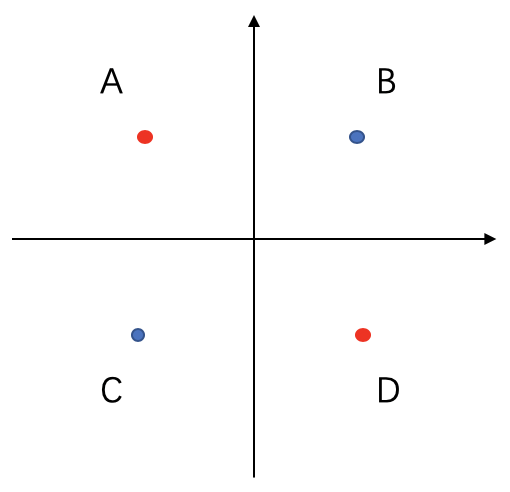
\includegraphics[width=4cm]{figs/XOR.png}\\
\caption{XOR}\label{fig4}
\end{wrapfigure}

前面讨论了生成模型(对数据有假设)和判别模型(计算)。都是在平面内线性可分的,考虑Fig.\ref{fig4}中的情况:若想要把AD分为一类,BC分为一类,显然在这个空间线性是不可分的饿,这时候就需要引入一个核方法(Kernel)。这种思想是用最简单的方法达到线性结果。

也就是从输入空间$\underset { \longrightarrow  }{ \phi  } $特征空间做一个非线性映射,$\phi :{ R }^{ p }\rightarrow { R }^{ r },\quad r\gg p$。让数据在跟高维的空间线性可分。$\phi(x)$作为特征,做一个线性模型。神经网络的做法是直接近似$\phi$,而核函数的方法是直接定义在这个特征空间里的内积形式,也就是只关心空间的内积性质,具体是什么空间,有什么其他其他性质并不关心。

定义$<\phi(x_1),\phi(x_2)>=k(x_1,x_2)$是两个数据点$x_1,x_2$的核函数。这个核函数的映射过程$k:R^p \times R^p \rightarrow R$必须满足两点性质:

1)$k(x,y)=k(y,x)$ 对称性
2)$k(x,y)\ge0$ 半正定性

常用的两种核函数是:

1)多项式核:$k(x,y)={1+<x,y>}^d$ 

2)高斯核:$k(x,y)=exp(-\frac { { \left\| x-y \right\|  }^{ 2 } }{ 2{ \sigma  }^{ 2 } } )$  ( $\phi(x)\in R^\infty $ ,因为可以拓展到无限维所以常用)

\textbf{例1:} 设$x,y\in R^2, d=2, x={(x_1,x_2)}^T, y={(y_1,y_2)}^T$。它的多项式核将2维扩展到6维:
\begin{equation}
\begin{aligned}
k(x,y) & ={(1+x_1y_1+x_2y_2)}^2\\ 
& ={x_1y_1}^2+{x_2y_2}^2+1+2x_1x_2y_1y_2+2x_1y_1+2x_2y_2\\ 
& =(1,\sqrt { 2 } { x }_{ 1 },\sqrt { 2 } { x }_{ 2 },\sqrt { 2 } { x }_{ 1 }{ x }_{ 2 },{ { x }_{ 1 } }^{ 2 },{ { x }_{ 2 } }^{ 2 }){ (1,\sqrt { 2 } { y }_{ 1 },\sqrt { 2 } { y }_{ 2 },\sqrt { 2 } { y }_{ 1 }{ y }_{ 2 },{ { y }_{ 1 } }^{ 2 },{ { y }_{ 2 } }^{ 2 }) }^{ T } \\ 
& =<\phi(x),\phi(y)>
\end{aligned}
\end{equation}

对于一个线性模型:$\sum _{ n=1 }^{ N }{ log(1+exp(-y_n{ w_n }^{ T }x_n))+\lambda { \left\| w \right\|  }^{ 2 } } $,

设有$\phi (x)\Rightarrow \sum _{ n=1 }^{ N }{ log(1+exp(-{ y }_{ n }{ ,\quad \phi ({ x }_{ n }) }>))+\lambda { \left\| w \right\|  }^{ 2 } } $,但是$\phi(x)$不知道,只知道$k(x_1,x_2)$。

\textbf{例2:} 设$x_1,x_2\in R$,对于一个高斯核
\begin{equation}
\begin{aligned}
k(x_1,x_2) & =exp(-\frac { { \left\| { x }_{ 1 }-{ x }_{ 2 } \right\|  }^{ 2 } }{ 2{ \sigma  }^{ 2 } } )\\ 
& =exp(-\frac { { \left\| { x }_{ 1 } \right\|  }^{ 2 }+{ \left\| { x }_{ 2 } \right\|  }^{ 2 }-2<{ x }_{ 1 },{ x }_{ 2 }> }{ 2{ \sigma  }^{ 2 } } )\\ 
& = exp(-\frac { { \left\| { x }_{ 1 } \right\|  }^{ 2 } }{ 2{ \sigma  }^{ 2 } } )exp(-\frac { { \left\| { x }_{ 2 } \right\|  }^{ 2 } }{ 2{ \sigma  }^{ 2 } }) exp(\frac { <{ x }_{ 1 },{ x }_{ 2 }> }{ { \sigma  }^{ 2 } } )\\ 
\end{aligned}
\end{equation}
\begin{equation}
\begin{aligned}
exp(\frac { <{ x }_{ 1 },{ x }_{ 2 }> }{ { \sigma  }^{ 2 } } )=\sum _{ k=0 }^{ \infty  }{ \frac { 1 }{ k! } { (\frac { <{ x }_{ 1 },{ x }_{ 2 }> }{ { \sigma  }^{ 2 } } ) }^{ k }=({ x }_{ 1 },{ { x }_{ 1 } }^{ 2 },...){ ({ x }_{ 2 },{ { x }_{ 2 } }^{ 2 },...) }^{ T } } \\ 
\end{aligned}
\end{equation}

这样高斯核就把二维数据扩展到无限维。

\subsection{Neural Network Methods}

\begin{wrapfigure}{r}{4.5cm}%靠文字内容的右侧
\includegraphics[width=3cm]{figs/fig5.png}
\caption{Neural Network}\label{fig5}
\end{wrapfigure}

现在看神经网络的解决方法。神经网络希望通过最简单的方法让X真实地表现出来。任意给定一个两层的神经网络,用ReLU做激活函数,假设输入的四个数据分别为{(1,1),(-1,-1),(-1,1),(1,-1)},设$h=(X^Tw+b)$,权重为$B=[[1,-1],[-1,1]]$,则通过一个ReLU的输出为

${ RelU }(X\cdot B)={ RelU }\left( \begin{array}{ll} { 0 } & { 0 } \\ { 0 } & { 0 } \\ { -2 } & { 2 } \\ { 2 } & { -2 } \end{array} \right) =\left( \begin{array}{l} { 0\quad 0 } \\ { 0\quad 0 } \\ { 0\quad 2 } \\ { 2\quad 0 } \end{array} \right) $

当再经过一个$(1,1)^T$的滤波,最后输出的结果是$(0,0,2,2)^T$,这样就把四个数据分开了。

\subsection{Underfit VS Overfit \& Bias VS Variance}

1. Underfit VS Overfit
\\

给定N个数据$\{x_1,...,x_N\}\in R^N$,$b_n\in R$,定义$y_n=f(x_n)_\epsilon_n$是一个预测器,其中$\epsilon_n$是噪音,且$E(\epsilon_n)=0,D(\epsilon_n)=\sigma^2$。预测器未知,通过数据找到一个估计$F(x)$尽可能与$f$接近,且在测试数据上表现良好。

a). F does poorly on training sample with large error $\rightarrow$ Underfitting

b). F does well on training sample but not well on testing sample $\rightarrow$ Overfitting

考虑${ \left\| Xb-y \right\|  }^{ 2 }$,X是一个$N\times P$的矩阵,若$N\gg P$,即数据个数远大于参数个数,容易造成underfit,反之若$N \ll P$,即参数个数远大于数据个数,容易造成overfit.
\\
\\2. Bias VS Variance
\\

$Bias = E(F(x)-f(x))$,若$Bias = 0$则$F(x)$是无偏的;若$Bias \neq 0$,但是当N趋近于无穷大时等于0,则是渐近无偏。

$Variance = E(E(x)-E^2(F(x))) = E(F(x))^2 - (E(F(X))^2)$

【欠拟合】:有偏

【过拟合】:方差很大

\begin{equation}
\begin{aligned} 
& \mathbb{E}\left((y-F(x))^{2}\right)\\ =&\left(\mathbb{E}(f(x)-F(x))^{2}+\mathbb{E}\left(\left(F(x)^{2}-\mathbb{E}(F(x))\right)^{2}\right)+\mathbb{E}(y-f(x))^{2}\right)\\
& \quad\quad\quad bias^2 \quad\quad\quad\quad variance \quad\quad\quad\quad\quad noise^2
\end{aligned}
\end{equation}

对于$F_\theta(x)$,$\theta$是未知的参数,利用$\{x_n\}$估计${\hat{\theta}_{N}=g\left(x_{1}, \cdots, x_{N}\right)}$统计量,

\begin{equation}
\begin{aligned}
& \text { bias }\left(\hat{\theta}_{N}\right)=\mathbb{E}\left(\hat{\theta}_{N}\right)-\theta \\
& \operatorname{Var}\left(\hat{\theta}_{N}\right)=\mathbb{E}\left(\hat{\theta}_{N}-E\left(\hat{\theta}_{N}\right)^{2}\right)\\
\end{aligned}
\end{equation}

若${x_1,...,x_N}\overset { iid }{ \sim  } bernulii(\theta) \sim \theta^{x}(1-\theta)^{1-x}$:

\begin{equation}
\hat{\theta}_{N}=\frac{1}{N} \sum_{n=1}^{N} x_{n} \quad E\left(\partial_{N}\right)=\frac{1}{N} \sum_{k=1}^{N} E\left(x_{n}\right)=\theta \text{无偏估计}
\end{equation}

若${x_1,...,x_N}\overset { iid }{ \sim  } Gaussian(\mu, \sigma^2)$:

\begin{equation}
\begin{aligned}
& \hat { \mu  } _{ N }=\frac { 1 }{ N } \sum _{ n=1 }^{ N }{ x_{ n } } \quad E\left( \hat { \mu  } _{ N } \right) =\mu \\
& \hat{\sigma}_{N}=\frac{1}{N} \sum_{n=1}^{N}\left(\chi_{n}-\hat{\mu}_{N}\right)^{2} \quad E\left(\hat{\sigma}_{N}\right)=\frac{N-1}{N} \sigma^{2} \text{渐近无偏}\\
& \hat{\sigma}_{N}=\frac{1}{N-1} \sum_{n=1}^{N}\left(x_{n}-\hat{\mu}_{N}\right)^{2} \text{无偏}\\
\end{aligned}
\end{equation}

\subsection{PCA}

设X是一个$N\times p$维的数据,定义$\phi(A,Z)=\frac_{1}_{2}tr((X-ZA^T)(X-ZA^T)^T)$,A是$p\times q$维矩阵,其中$q<p$,A是列正交的,即$A^A=I_q$。这时我们称A是投影矩阵,Z是一个低维表示。我们的目标是找到A和Z,然后$\underset {Z,A}{min} \varphi (A,Z)$,也就是最小化${\left\| X-Z{ A }^{ T }\right\|}_{ F }^{ 2 }$,若找到$A_{p\times q}$,有$min(X-XAA^T)$最小即可。

定义Lagrange函数$(A,Z)=\frac { 1 }{ 2 } tr((X-Z{ A }^{ T }){ (X-Z{ A }^{ T }) }^{ T })-\frac { 1 }{ 2 } tr(L({ A }^{ T }A-{ I }_{ q }))$,$A=[a_1,..,a_q]^T$,L是拉格朗日乘子矩阵,是个对称阵,则要找$\frac_{dL}_{dA}=0,\frac_{dL}_{dZ}=0$的解。

\begin{equation}
\begin{aligned}
dL & =\frac { 1 }{ 2 } { tr }\left( d\left( XA^{ T } \right) \left( X-ZA^{ T } \right) ^{ T } \right) +\frac { 1 }{ 2 } { tr }\left( X-ZA^{ T } \right) d\left( X-ZA^{ T } \right) ^{ \top  })-\frac { 1 }{ 2 } { tr }\left( L(dA^{ T }A+A^{ T }dA \right) \\ 
& =...+...-\frac { 1 }{ 2 } (tr(LdA^{ T }A)+tr(LA^{ T }dA))\\
& =...+...-\frac { 1 }{ 2 } (tr(ALdA^{ T })+tr(dA^{ T }AL))\\ 
& =...+...-\frac { 1 }{ 2 } (tr(ALdA^{ T })+tr(ALdA^{ T }))\quad \quad (tr(AB)=tr(BA))\\ 
& ={ tr }\left( (X-ZA^{ T })d{ (X-ZA^{ T }) }^{ T } \right) -tr(ALdA^{ T })\\ 
& ={ tr }\left( X-ZA^{ T } \right) (AdZ^{ T }+dAZ^{ T })-tr(ALdA^{ T })\\ 
& =tr(\left( X-ZA^{ T } \right) AdZ^{ T })+tr(X-ZA^{ T })dAZ^{ T })-tr(ALdA^{ T })\\
& =...+tr(ZdA^{ T }{ \left( X-ZA^{ T } \right)  }^{ T })-...\\ 
& =...+tr(\left( X-ZA^{ T } \right) ZdA^{ T })-...\\ 
& =-tr((X-ZA^{ T })A(dZ^{ T }))-tr((X^{ T }Z-AZ^{ T }Z+AL)dA^{ T })\\
\end{aligned}
\end{equation}

\begin{equation}
\begin{aligned}
\left\{\begin{array}{l}{\frac{d L}{d Z}=-\left(X-2 A^{T}\right) A=0} \\ 
{\frac{d L}{d A}=-\left(X^{T} Z-A Z^{T} Z+A L\right)=0} \\ 
{A^{T} A-I_q=0}\end{array}\right.
\end{aligned}
\end{equation}

解方程:

\begin{equation}
\begin{aligned}
(X-ZA^T) A=0 & \Rightarrow Z=XA \\
X^Z-AZ^TZ+AL=0 & \Rightarrow A^TX^Z-A^TAZ^TZ+A^TAL=0\\
& \quad L=Z^Z-A^TX^Z\\
& \Rightarrow X^TXA=AA^TX^TXA
\end{aligned}
\end{equation}

对$A^TX^T X A$可以做特征值分解写成$S\Lambda S^T$,$X^T X A=AS\LambdaS^T$,$X^T X A S=A S\Lambda$,$AS$是特征向量,$\Lambda$是特征值。

回到开始的问题$\underset {Z,A}{min} \varphi (A,Z)$,设$Z=XA$,

\begin{equation}
\begin{aligned}
min \phi & = min tr((X-XA^T)(X-XA^T)^T)\\
& = min tr(X(I-AA^T)X^T)\\
& = min tr(XX^T)-tr(XAA^TX^T)\\
& = ...-tr(A^TX^TXA)\\
& = ...-tr(\Lambda)\\
& = tr(XX^T)-tr(\Lambda)\\
\end{aligned}
\end{equation}

则$\Lambda$为$XX^T$的最大前q个特征值才能让$\phi$最小,AS是对应的特征向量。


\section{Neural Network}
\subsection{Six Keys}
神经网络的基本思想是想要找一个$F(x)$来逼近函数$f(x)$,用复合形式来找:$F=F_L(F_{L-1}...())$。其中有六个关键:

1. Key Compound Operation 

2. Key Chain Rule 

3. Key Architecture (CNN/RNN)

4. Key Algorithm (SGD)

5. Key Subroutine (Back-Propagation to execute the channel)

6. Key Nonlinear (ReLU)



\end{document}
